% vim: set ts=2 sw=2 noet:
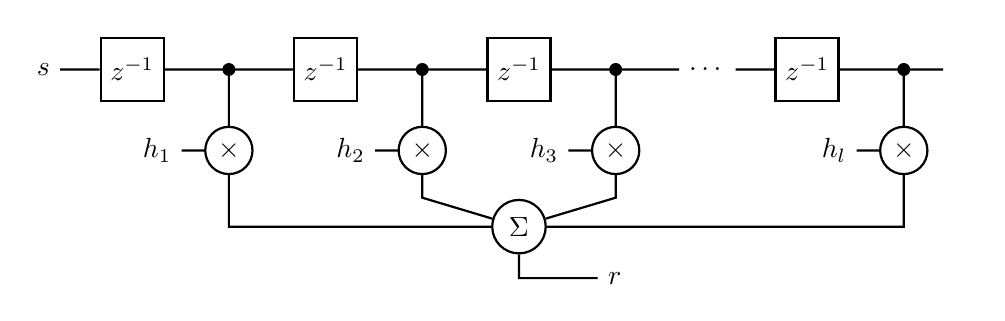
\begin{tikzpicture}[
		dot/.style = {
			circle,
			fill = black, draw = black,
			minimum size = 1.5mm,
			outer sep = 0, inner sep = 0,
		},
		block/.style = {
			rectangle, draw, thick,
			black, fill = white,
			minimum height = 8mm, minimum width = 8mm,
		},
		prod/.style = {
			circle, draw, thick,
			black, fill = white,
			minimum size = 6mm,
			inner sep = 0, outer sep = 0,
		},
		sum/.style = {
			circle, draw, thick,
			black, fill = white,
			minimum size = 4mm,
		},
	]

	\matrix[column sep = 5mm, row sep = 3mm] {
		\node[block] (B0) {\(z^{-1}\)}; & \node[dot] (D0) {}; &
		\node[block] (B1) {\(z^{-1}\)}; & \node[dot] (D1) {}; &
		\node[block] (B2) {\(z^{-1}\)}; & \node[dot] (D2) {}; & \node (dots) {\ldots}; & 
		\node[block] (Bk) {\(z^{-1}\)}; & \node[dot] (Dk) {};
		\\
		& \node[prod] (P0) {\(\times\)}; &
		& \node[prod] (P1) {\(\times\)}; &
		& \node[prod] (P2) {\(\times\)}; & &
		& \node[prod] (Pk) {\(\times\)}; &
		\\
		& & & & \node[sum] (S) {\(\Sigma\)}; \\
	};

	\draw[thick]
		% tapped delayed line
		(B0.west) -- ++(-5mm,0) node[left] {\(s\)}
		(B0.east) -- (D0) -- (B1.west)
		(B1.east) -- (D1) -- (B2.west)
		(B2.east) -- (D2) -- (dots) -- (Bk.west) 
		(Bk.east) -- (Dk) -- ++(5mm,0)
		% taps asd sum
		(D0) -- (P0) |- (S)
		(D1) -- (P1) -- ++(0,-6mm) -- (S)
		(D2) -- (P2) -- ++(0,-6mm) -- (S)
		(Dk) -- (Pk) |- (S)
		% product weights
		(P0.west) -- ++(-3mm,0) node[left] {\(h_1\)}
		(P1.west) -- ++(-3mm,0) node[left] {\(h_2\)}
		(P2.west) -- ++(-3mm,0) node[left] {\(h_3\)}
		(Pk.west) -- ++(-3mm,0) node[left] {\(h_l\)}
		% result
		(S.south) |- ++(1cm,-3mm) node[right] {\(r\)}
	;

\end{tikzpicture}
